\documentclass[
    TIC, % Saisir le nom de l'institut rattaché
    il, % Saisir le nom de l'orientation
    % confidential, % Décommentez si le travail est confidentiel
]{heig-tb}

\usepackage[nooldvoltagedirection,european,americaninductors]{circuitikz}

\signature{iescher.svg} % Remplacer par votre propre signature vectorielle.

\makenomenclature
\makenoidxglossaries
\makeindex

\addbibresource{bibliography.bib}

\input{nomenclature}
\input{acronyms}
\newglossaryentry{heig-vd}{
    name=HEIG-VD,
    description={Haute École d'Ingénierie et de Gestion du canton de Vaud}
}
\newglossaryentry{hes-so}{
    name=HES-SO,
    description={Haute École Supérieure de Suisse Occidentale}
}
\newglossaryentry{latex}{
    name=latex,
    description={Un langage et un système de composition de documents}
}
\newglossaryentry{maths}{
    name=mathematics,
    description={Les mathematiques sont ce que les mathématiciens fonts}
}
\newglossaryentry{géométrie}{
    name=géométrie,
    description={Une structure de donnée contenant plusieurs points et formant un polygone}
}
\newglossaryentry{tags}{
    name=tags,
    description={Objets contenus par une entité de la base de donnée OpenStreetMap servant à stocker des informations supplémentaires. Non obligatoires.}
}
\newglossaryentry{OSM}{
    name=OSM,
    description={OpenStreetMap}
}
\newglossaryentry{implicit tiling}{
    name=implicit tiling,
    description={Une technique qui consiste à diviser la carte en tuiles de manière récursive.}
}
% Auteur du document (étudiant-e) en projet de Bachelor
\author{Ian Escher}

% Activer l'option pour l'accord du féminin dans le texte
\genre{male}

% Titre de votre travail de Bachelor
\title{Tuilage de données géospatiales pour le métaverse}

% Le sous titre est optionnel
\subtitle{Travail de Bachelor}

% Nom du professeur responsable
\teacher {Prof. B. Chapuis (HEIG-VD)}

% Mettre à jour avec la date de rendu du travail
\date{25.07.2024}

% Numéro de TB
\thesis{7265}


\usepackage{listings}
\usepackage{xcolor}

% Define the style for Java code
\lstdefinestyle{java}{
  language=Java,
  basicstyle=\ttfamily\footnotesize,
  keywordstyle=\color{blue},
  commentstyle=\color{gray},
  stringstyle=\color{red},
  numbers=left,
  numberstyle=\tiny\color{gray},
  stepnumber=1,
  numbersep=4pt,
  showstringspaces=false,
  tabsize=4,
  breaklines=true,
  breakatwhitespace=false,
  escapeinside={(*@}{@*)},
}

% \begin{document}

% \section{Example Java Code}

% Here is an example of Java code:

% \begin{lstlisting}[style=java]
% public class HelloWorld {
%     public static void main(String[] args) {
%         // Prints "Hello, World" to the terminal window.
%         System.out.println("Hello, World");
%     }
% }
% \end{lstlisting}

% \end{document}

\surroundwithmdframed{minted}

%% Début du document
\begin{document}
\selectlanguage{french}
\maketitle
\frontmatter
\clearemptydoublepage

%% Requis par les dispositions générales des travaux de Bachelor
\preamble
\authentification

%% Résumé / Résumé publiable / Version abrégée
\begin{abstract}
    Le travail devant être effectué durant ce travail consiste à utiliser la spécification \href{https://cesium.com/blog/2021/11/10/introducing-3d-tiles-next/}{3D Tiles Next}\footnote{https://cesium.com/blog/2021/11/10/introducing-3d-tiles-next/} de \href{https://cesium.com/}{Cesium}\footnote{https://cesium.com/} pour \textit{streamer} un rendu 3D de tuiles vectorielles à l'intérieur du \href{https://github.com/baremaps/baremaps}{framework Baremaps}\footnote{https://github.com/baremaps/baremaps} existant. Le produit final sera un prototype du support de cette spécification en utilisant une base de données \href{https://postgis.net/}{Postgis}\footnote{https://postgis.net/}. Les fonctionnalités offertes 3D Tiles Next seront pleinement utilisées pour produire un rendu de haute qualité et performant.

Les rendus 3D que propose Cesium peuvent être distribués en deux catégories :

\begin{itemize}
    \item[1.] Le terrain géographique
    \item[2.] Les bâtiments
\end{itemize}

Produire le rendu du terrain ainsi que le rendu des bâtiments comporte chacun ses propres difficultés d'optimisation. Un système de \textit{level of details} devra être implémenté pour maintenir de hautes performances, même avec un nombre important de géométries affichées à l'écran.

Cependant, dans le cadre de ce travail, seul l'affichage des bâtiments sera traité. Pour cela, la spécification 3D Tiles Next propose une solution d'optimisation interne à son fonctionnement avec Cesium. Néanmoins, beaucoup reste à être fait quant à l'affichage des bâtiments ainsi que pour créer un système permettant de \textit{streamer} les informations de la base de données d'OpenStreetMap vers Cesium.

% \asterism

\end{abstract}

%% Sommaire et tables
\clearemptydoublepage
{
    \tableofcontents
    \let\cleardoublepage\clearpage
    \listoffigures
    \let\cleardoublepage\clearpage
    % \listoftables
    % \let\cleardoublepage\clearpage
    % \listoflistings
}

\printnomenclature
\clearemptydoublepage
\pagenumbering{arabic}

%% Contenu
\mainmatter


\chapter{Introduction}
% L'introduction est une section requise dans un rapport technique. Introduisez votre travail, l'idée de départ et les objectifs attendus. Un lecteur qui découvrirait votre projet au travers de cette introduction devrait ainsi être capable d'en comprendre le cadre, l'idée générale et les aboutissants du projet.

Durant ce travail, j'ai écrit un programme sur la base du \href{https://github.com/baremaps/baremaps}{framework Baremaps}\footnote{https://github.com/baremaps/baremaps} permettant à un client \href{https://cesium.com/}{Cesium}\footnote{https://cesium.com/} d'obtenir les ressources nécessaires à afficher les bâtiments du dataset d'\href{https://www.openstreetmap.org/}{OpenStreetMap}\footnote{https://www.openstreetmap.org/} en 3D.

Ces ressources utilisent la spécification \href{https://cesium.com/blog/2021/11/10/introducing-3d-tiles-next/}{3D Tiles Next}\footnote{https://cesium.com/blog/2021/11/10/introducing-3d-tiles-next/} de Cesium tout en respectant la version 1.1 de leur \href{https://docs.ogc.org/cs/22-025r4/22-025r4.html}{standard de tuiles vectorielles}\footnote{https://docs.ogc.org/cs/22-025r4/22-025r4.html}. Cette nouvelle version de leur spécification introduit entre autre la fonctionnalité de \textit{implicit tiling} \cite{implicit-tiling-gh} qui permet une utilisation facilitée de datasets volumineux. Les ressources qui seront fournies au client Cesium utiliseront donc cette fonctionnalité.

Le programme se divise en deux parties : la première est celle qui s'occupe de la génération des tuiles vectorielles contenant les bâtiments d'OpenStreetMap en 3D et la seconde est celle qui va construire les \textit{Subtrees}, des objects indispensables au client Cesium pour optimiser l'affichage des tuiles. Ces deux parties ne sont pas équivalentes en termes de complexité. La première est plus simple et a été réalisée en premier. La seconde a nécessité d'avantages d'études ainsi que le développement de plusieurs algorithmes pour être implémentée.

Tout le code source de ce projet peut être trouvé sur mon projet GitHub à l'adresse : \href{https://github.com/IEscher/incubator-baremaps-TB-ian}{https://github.com/IEscher/incubator-baremaps-TB-ian}

\newpage
\section*{Fondements écrits par Antoine Drabble}

Afin d'évaluer si le projet s'apprêtais à être utilisé dans le cadre d'un travail de Bachelor, M. Antoine Drabble a effectué un travail de recherche et a produit un prototype de visualisation de bâtiments 3D à l'intérieur du client Cesium JS sur lequel je vais m'appuyer. Ce prototype, bien qu'incomplet, pose les fondements de l'utilisation de Cesium JS, de la spécification 3D Tiles et du framework Baremaps les uns avec les autres. Ce prototype est donc un bon point de départ pour mon travail.

% \section{Contexte}
% Cette section \underline{n'est pas obligatoire}, mais elle est souvent présente dans un rapport technique pour compléter l'introduction et définir le contexte du travail \cad le cadre formel dans lequel le travail est mené.

%%if
% \section{Citations et bibliographie}
% Citer vos sources est essentiel. Avec \texttt{biblatex} vous pouvez facilement citer des articles, des livres ou des sites internet. Toutes les citations dans le texte seront automatiquement regroupées en fin de document dans la section \guillemotleft Bibliographie\guillemotright. Par exemple, citons un article d'Einstein \cite{einstein} ou le livre de Dirac \cite{dirac}.

% Parfois il peut être utile d'utiliser un gestionnaire de bibliographie. La communauté académique recommande l'outil \href{https://www.zotero.org/}{Zotero} qui permet de gérer une bibliothèque numérique d'ouvrages et de références numériques. Il permet également de générer une bibliographie compatible avec \LaTeX.

% Notez qu'il est très facile d'obtenir l'extrait \texttt{bibtex} depuis des journaux. Sélectionnez \emph{export/citation}. Si vous le pouvez choisissez \texttt{bibtex}. Dans le cas d'un format \texttt{.ris}, utilisez un convertisseur en ligne comme \href{http://www.bruot.org/ris2bib/}{ris2bib}.

% \section{Adapter votre modèle}
% Ce document n'est qu'un modèle ayant pour but de revoir les quelques avantages de \LaTeX~ et les fonctionnalités qui pourraient vous être utiles pour rédiger un rapport académique. N'hésitez pas à supprimer les parties inutiles et à adapter ce modèle à vos besoins.
%%fi

\chapter{3D Tiles}

\section{Spécification 3D Tiles Next}
\label{sec:3d-tiles-next}
La spécification \href{https://cesium.com/blog/2021/11/10/introducing-3d-tiles-next/}{3D Tiles Next}\footnote{https://cesium.com/blog/2021/11/10/introducing-3d-tiles-next/} de \href{https://cesium.com/}{Cesium}\footnote{https://cesium.com/} est une spécification open source permettant de visualiser des données géospatiales en 3 dimensions.

Pour pouvoir être utilisé, un dataset de données géospatiales doit être partitionné car il est souvent trop complexe pour nos ordinateurs de le traiter en entier. Cette spécification décrit comment le faire en organisant ces données en \textit{Tiles} et en \textit{Tilesets} pour pouvoir ensuite être fournies à un client tel que Cesium. Les Tiles, ou tuiles, contiennent toutes les informations nécessaires à décrire une portion d'une database dans un espace 3D comme par exemple un \textit{bounding volume} qui décrit le volume 3D de la tuile ou encore son \textit{content} qui contient l'objet 3D à afficher. Une Tile contient aussi une liste de Tile appellée \textit{children}. Un Tilesets possède diverses informations comme la version de la spécification utilisée mais aussi une liste de Tile tout comme les Tiles. Cette structure permet de diviser les données en une hiérarchie de Tiles en arbre, ce qui facilite la recherche et le traitement des données.

\begin{figure}[H]
    \centering
    \includegraphics[width=0.8\textwidth]{assets/figures/Tilesets.png}
    \caption{Exemple de Tileset contenant un arbre de Tiles \cite{3d-tiles-reference-card-v1}}
    \label{fig:Tilesets}
\end{figure}

D'autres éléments sont présents dans les Tiles et Tilesets. Certains seront abordés plus tard dans ce rapport, sinon, pour plus d'informations sur la spécification 3D Tiles, vous pouvez consulter les \href{https://github.com/CesiumGS/3d-tiles/tree/main/reference-cards}{documents de références proposés par Cesium}\footnote{https://github.com/CesiumGS/3d-tiles/tree/main/reference-cards}.

\section{Implicit Tiling}
\label{sec:implicit-tiling}
\subsection{Nouveautés de la version 1.1 de 3D Tiles}

Avec la nouvelle version 1.1 de la spécification 3D Tiles, il a été introduit une nouvelle fonctionnalitée appelée \textit{Implicit Tiling}. Elle permet de diviser implicitement un dataset en tuiles de mêmes tailles sans avoir à les définir explicitement.

Pour cela, l'implicit tiling divise la carte en tuiles de manière récursive. Tant que le \texttt{level} de division n'a pas atteint la valeur maximum \texttt{availableLevels}, on divise la tuile dans laquelle nous nous trouvons en tuiles de même taille.

Deux méthodes de division sont actuellement disponibles : \texttt{QUADTREE} et \texttt{OCTREE}. La première reste sur un concept de tuiles en deux dimensions, tandis que les octrees permettent de diviser les tuiles en rajoutant une notion de hauteur, donc en 3 dimensions. Dans mon cas, j'utilise une division en quadtree puisque tout les bâtiments que je dois traiter se trouvent sur un plan 2D.

\begin{figure}[H]
    \centering
    \includegraphics[width=0.6\textwidth]{assets/figures/implicit-tiling-small.png}
    \caption{Division en quadtree par implicit tiling \cite{3d-tiles-specification}}
    \label{fig:implicit-tiling}
\end{figure}

Le niveau 0 englobe l'entièreté du Tileset, dans notre cas la planète entière, puis, à chaque division, chaque tuile correspond non pas à une profondeur supplémentaire, mais à une portion de plus en plus petite du Tileset. Ainsi, une tuile de \texttt{level} 0 est la tuile de base, une tuile de \texttt{level} 1 est une tuile résultant de la division de la tuile de \texttt{level} 0, etc. Plus d'informations quand à l'indexation des tuiles sont disponibles dans la section \ref{sec:morton}.

Pour définir un implicit tiling, il faut en premier lieux créer un Tileset hôte qui définira entre autre son \texttt{bounding volume}. L'implicit tiling va ensuite définir les tuiles de ce Tileset hôte en fonction de son \texttt{subdivisionScheme}, de son \texttt{subtreeLevels} et de ses \texttt{availableLevels}, tout en prenant comme taille initiale le \texttt{bounding volume} du Tileset. Enfin, il est possible de définir les adresses auxquelles le clien doit envoyer des requêtes pour obtenir les tuiles.

En plus de l'implicit tiling, la version 1.1 de 3D Tiles apporte le support des fichiers GLTF ainsi que deux nouvelles extensions : \href{https://github.com/CesiumGS/glTF/tree/3d-tiles-next/extensions/2.0/Vendor/EXT_mesh_features}{EXT_mesh_features}\footnote{https://github.com/CesiumGS/glTF/tree/3d-tiles-next/extensions/2.0/Vendor/EXT_mesh_features} et \href{https://github.com/CesiumGS/glTF/tree/3d-tiles-next/extensions/2.0/Vendor/EXT_structural_metadata}{EXT_structural_metadata}\footnote{https://github.com/CesiumGS/glTF/tree/3d-tiles-next/extensions/2.0/Vendor/EXT_structural_metadata}. Cela introduit beaucoup de nouvelles possibilités par rapport à l'ancien système, notamment à des \textit{metadata} très précises par objet GLTF. 

Bien que la génération de fichiers GLTF sera discuté dans la section \ref{sec:gltf}, je ne parlerai pas des extensions dans ce rapport puisqu'elles n'ont pas été utilisées dans mon projet.

\subsection{Avantages et inconvénients de l'implicit tiling}

Comme son nom l'indique, cette technique de division de tuiles est implicite, ce qui signifie que l'on ne peut pas définir nous même les caractéristiques des tuiles. Cela peut être un avantage pour des datasets très grands, comme une planète entière, où il serait difficile de définir explicitement les tuiles, mais cela peut poser problème lorsque le \texttt{bounding volume} d'une tuile contenant une petite maison de campagne sera le même que celui de la tuile qui contiendra l'Empire State Building. LODSSSS ????

\section{Level of Detail}
\label{sec:lod}
Les \textit{Level Of Details}, appellés aussi LOD, est une technique qui permet de définir plusieurs niveaux de détails pour un même objet 3D. Cela permet de charger des objets plus ou moins détaillés en fonction de la distance à laquelle ils se trouvent de la caméra. Grâce à cela, il est possible de réduire la charge de travail de l'ordinateur en ne chargeant que le niveau de détail nécessaire pour garder un rendu qui, à l'oeil humain, semble identique à celui d'un contenant tous les objets entièrement détaillés.

Pour calculer le bon niveau de détail à afficher, Cesium utilise le \texttt{bounding volume} ainsi que le \texttt{geometric error} d'une tuile. Le concept est simple, plus un objet occupe une partie importante de la fenêtre de rendu, plus il doit être détaillé. Le \textit{Screen Space Error} ou SSE est une valeur qui permet de déterminer l'imprécision du rendu d'un objet en Pixels. Grâce à elle, il nous est possible de déterminer un seuil SSE auquel Cesium devra changer de LOD. Pour déterminer ce seuil, il nous est possible de définir un \texttt{geometric error} pour chaque tuile. Ce \texttt{geometric error} est une valeur qui permet de déterminer la distance maximale entre la géométrie réelle et la géométrie simplifiée en mètres. Plus cette valeur est grande, plus la géométrie simplifiée sera éloignée de la géométrie réelle. Avec le \texttt{geometric error}, le \texttt{bounding volume} et la distance entre la caméra et l'objet, il est possible de déterminer le SSE d'une tuile selon la formule suivante :

\begin{equation}
    \centering
    SSE = \frac{geometricError}{distance} \times \frac{screenHeight}{\tan(fovy/2)}
\end{equation}

Où \texttt{screenHeight} est la hauteur de la fenêtre de rendu en pixels et \texttt{fovy} est l'angle de vue de la caméra en radians sur l'axe des y.

Pour plus d'informations, vous pouvez consulter la spécification 3D Tiles \cite{3d-tiles-specification}. Des graphiques tels que celui de la figure \ref{fig:sse} sont disponibles pour mieux comprendre le concept.

\begin{figure}[H]
    \centering
    \includegraphics[width=1\textwidth]{assets/figures/sse.png}
    \caption{Calcul du SSE \cite{3d-tiles-specification}}
    \label{fig:sse}
\end{figure}

\section{3DTILES\_bounding\_volume\_S2 extension}
\label{sec:3DTILES_bv_S2}
Lors de la section sur l'implicit tiling \autoref{sec:implicit-tiling}, j'ai mentionné que l'implicit tiling créait les \texttt{bounding volumes} et les \texttt{geometric errors} de manière automatique. Ce n'est pas vraiment le cas. Par défaut, ils ne sont pas définis par l'implicit tiling, mais il est possible de rajouter l'extension \href{https://github.com/CesiumGS/3d-tiles/tree/main/extensions/3DTILES_bounding_volume_S2}{3DTILES\_bounding\_volume\_S2}\footnote{https://github.com/CesiumGS/3d-tiles/tree/main/extensions/3DTILES\_bounding\_volume\_S2} qui permet de compléter les tuiles générées par l'implicit tiling avec des \texttt{bounding volumes} et des \texttt{geometric errors} calculés automatiquement.

Sans trop rentrer dans les détails, l'extension utilise une \href{https://en.wikipedia.org/wiki/Hilbert_curve}{courbe de Hilbert}\footnote{https://en.wikipedia.org/wiki/Hilbert\_curve} sur une partition en plusieurs niveaux de tuiles faite par la librairie \href{http://s2geometry.io/}{S2 Geometry}\footnote{http://s2geometry.io/}. Ce sujet rentre dans la thématique des \href{https://en.wikipedia.org/wiki/Binary_space_partitioning}{Binary Space Partitioning}\footnote{https://en.wikipedia.org/wiki/Binary\_space\_partitioning}. Tout comme la partition du monde en 2 dimensions et son indexation avec un index de Motron qui sera vu dans la section \ref{sec:morton}, le partitionnement du monde peut aussi se faire avec la librairie S2 Geometry et son indexation avec une courbe de Hilbert. Ces deux méthodes sont donc des \textit{Binary Space Partitioning}. Ici, ces méthodes permettent de diviser une surface et permettent de donner rapidement et efficacement les informations spatiales des tuiles.

Pour utiliser cette extension, il suffit de rajouter les champs \texttt{extensionsUsed} et \texttt{extensionsRequired} dans le fichier JSON du Tileset. Puis, il faut rajouter une tuile dans le champ \texttt{children} du fichier JSON du Tileset. Cette tuile doit contenir un champ \texttt{boundingVolume} avec un champ \texttt{extensions} contenant les informations nécessaires pour l'extension.

Remarquez le champ \texttt{token} dans l'exemple ci-dessous. Il s'agit d'un identifiant unique correspondant à la \textit{root cell} (la cellule de plus haut niveau) de la courbe de Hilbert. Selon l'extension, le globe terrestre à été divisé en 6 \textit{root cells} comme si l'on avait projeté les 6 faces d'un cube sur la terre. Par exemple, l'Antarctique se trouve dans la cellule "5".

\newpage

Voici un exemple de fichier JSON utilisant l'extension 3DTILES\_bounding\_volume\_S2 :

\begin{verbatim}
{
    "asset" : {
        "version" : "1.1"
    },
    "geometricError": 1200000,
    "extensionsUsed": [
        "3DTILES_bounding_volume_S2"
    ],
    "extensionsRequired": [
        "3DTILES_bounding_volume_S2"
    ],
    "root" : {
        "boundingVolume": {
        "region": [-3.14159, -1.57079, 3.14159, 1.57079,
            0, 60
        ]
        },
        "refine": "REPLACE",
        "geometricError": 1200000,
        "children": [
        {
            "boundingVolume": {
            "extensions": {
                "3DTILES_bounding_volume_S2": {
                "token": "1",
                "minimumHeight": 0,
                "maximumHeight": 20
                }
            }
            },
            "refine": "REPLACE",
            "geometricError": 120000
        },
        ],
        "content": {
            "uri" : "/content/content_glb_{level}__{x}_{y}.glb"
        },
        "implicitTiling" : {
            "subdivisionScheme" : "QUADTREE",
            "subtreeLevels" : 4,
            "availableLevels" : 19,
            "subtrees" : {
                "uri" : "/subtrees/{level}.{x}.{y}.subtree"
            }
        }
    }
}
\end{verbatim}

\begin{figure}[H]
    \centering
    \includegraphics[width=1\textwidth]{assets/figures/s2cell_global.jpg}
    \caption{Tokens des 6 \textit{root cells} \cite{3DTILES_bounding_volume_S2-website}}
    \label{fig:s2-ext}
\end{figure}

Notez aussi que dans l'exemple JSON ci-dessus, qu'une seule \textit{root cell} est définie. Dans mon cas, comme j'aimerai pouvoir utiliser l'entièreté de la terre, j'ai défini les 6 \textit{root cells} en tant que 6 \texttt{children} différents avec chacun leur propre \texttt{token}.

Cette manière de partager l'espace de la terre ne correspond cependant pas à la méthode qu'utilise l'implicit tiling. Les calculs nécessairs pour convertir les indexes de l'implicit tiling vers ceux des courbes de Hilbert ne sont néanmoins pas à effectuer par nos soins, l'extension ce charge de cela.

\section{Création des fichiers glTF}
\label{sec:gltf}
Grâce à l'introduction du support des fichiers glTF ou plus précisément des fichiers glb dans la spécification 3D Tiles 1.1, il est devenu beaucoup plus facile de générer des fichiers 3D comparé à l'ancien système. Ici, j'utilise la librairie \href{https://github.com/javagl/JglTF}{jglTF}\footnote{https://github.com/javagl/JglT} et la librairie \href{https://locationtech.github.io/jts/}{JTS}\footnote{https://locationtech.github.io/jts/} pour créer les \textit{nodes}, les \textit{meshes}, les \textit{materials} et les textures des bâtiments. Toute la logique concernant la création des fichiers glTF se trouve dans la classe \texttt{GltfBuilder}\footnote{baremaps-core/src/main/java/org/apache/baremaps/tdtiles/GltfBuilder.java}.

\subsection{Système de compression des géométries des bâtiments}

Comme vu à la section \ref{sec:lod}, il est nécessaire de pouvoir fournir plusieurs niveaux de détails en fonction du niveau de la tuile. Pour cela, j'ai implémenté un système de compression des géométries des bâtiments. Ce système se base sur les \texttt{levels} des tuiles discutés à la section \ref{sec:implicit-tiling}. Plus le \texttt{level} est élevé, plus les bâtiments sont proches de la caméra et donc plus les bâtiments doivent être détaillés. Pour effectuer la compression, j'utilise la class \href{https://locationtech.github.io/jts/javadoc/org/locationtech/jts/simplify/TopologyPreservingSimplifier.html}{\textit{TopologyPreservingSimplifier}}\footnote{https://locationtech.github.io/jts/javadoc/org/locationtech/jts/simplify/TopologyPreservingSimplifier.html} de la librairie \texttt{org.locationtech.jts} qui permet de simplifier une géométrie en fusionnant les points les plus proches d'une géométrie.

En fonction du niveau de compression de leur tuile, les bâtiments subissent jusqu'à 3 niveau de compression :

\begin{itemize}
    \item niveau de compression 0 : Les bâtiments sont affichés avec toutes les géométries.
    \item niveau de compression 1 : Les bâtiments sont affichés avec une géométrie légèrement simplifiée.
    \item niveau de compression 2 : Les bâtiments sont affichés avec une géométrie très simplifiée.
    \item niveau de compression 3 : Les bâtiments sont affichés avec une géométrie très simplifiée uniquement si ils ont des caractéristiques spécifiques enregistrées dans la base de données OSM.
\end{itemize}

Pour visualiser les différences entre les niveaux de compression, je vous invite à regarder les figures ci-dessous où chaque niveau de détail est symbolisé par une couleur :

\begin{itemize}
    \item niveau de compression 0 : rouge
    \item niveau de compression 1 : jaune
    \item niveau de compression 2 : vert
    \item niveau de compression 3 : bleu
\end{itemize}


\begin{figure}[H]
    \centering
    \includegraphics[width=1\textwidth]{assets/figures/lods-horizon.png}
    \caption{Vue à l'horizon de la ville de Londres}
    \label{fig:lods-horizon}
\end{figure}

\begin{figure}[H]
    \centering
    \begin{minipage}{0.49\textwidth}
        \centering
        \includegraphics[width=\textwidth]{assets/figures/lods0.png}
        \caption{Level 0}
        \label{fig:lods0}
    \end{minipage}\hfill
    \begin{minipage}{0.49\textwidth}
        \centering
        \includegraphics[width=\textwidth]{assets/figures/lods1.png}
        \caption{Level 1}
        \label{fig:lods1}
    \end{minipage}
    \vspace{1cm}
    \begin{minipage}{0.49\textwidth}
        \centering
        \includegraphics[width=\textwidth]{assets/figures/lods2.png}
        \caption{Level 2}
        \label{fig:lods2}
    \end{minipage}\hfill
    \begin{minipage}{0.49\textwidth}
        \centering
        \includegraphics[width=\textwidth]{assets/figures/lods3.png}
        \caption{Level 3}
        \label{fig:lods3}
    \end{minipage}
\end{figure}


Faire ainsi permet de réduire drastiquement le temps passé à générer ces bâtiments ainsi que de garantir un affichage plus fluide chez le client tout en gardant une qualité d'affichage correcte.

Outre la compression des géométries, une autre optimisation qui pourrait être développée est un filtrage des tuiles en fonction de leur quantité de bâtiments et de leur niveau de compression. Par exemple, une tuile qui ne contient qu'un ou deux petits bâtiments pourrait être omise à l'affichage, si elle se trouve assez loin de la caméra pour être à un niveau de compression élevé.

\subsection{Géométries des bâtiments}

Avec le niveau de compression ainsi que la \texttt{Geometry}\footnote{org.locationtech.jts.geom.Geometry}, qui nous sert à déterminer le polygone au sol du bâtiment, nous pouvons extruder le bâtiment en 3D. Cependant une \texttt{Geometry} ne contient qu'une liste de points et il faut une liste de triangles pour pouvoir modéliser le bâtiment en 3D. Pour cela, il faut une méthode qui fonctionne avec des polygones concaves et qui déforme le moins possible les géométrie des bâtiments. Une méthode faisant explicitement cela est la méthode \texttt{simplify} de la classe \textit{TopologyPreservingSimplifier} qui fonctionne avec des polygones concaves et qui, comme son nom l'indique, préserve la topologie initiale de la géométrie. Cette librairie \texttt{org.locationtech.jts} propose aussi la classe \href{https://locationtech.github.io/jts/javadoc/org/locationtech/jts/triangulate/polygon/PolygonTriangulator.html}{\texttt{PolygonTriangulator}}\footnote{https://locationtech.github.io/jts/javadoc/org/locationtech/jts/triangulate/polygon/PolygonTriangulator.html} qui permet aussi de faire une triangulation de polygones concaves de manière moins optimisée mais plus rapide que la classe \textit{TopologyPreservingSimplifier}. Elle pourrait donc aussi être utilisée pour générer les bâtiments en 3D si souhaité.

Grâce à cette triangulation, il est possible de modéliser les bâtiments en 3D correctement, même ceux comprenant des cours intérieures ou des trous dans leur structure.

La classe \texttt{TopologyPreservingSimplifier} comporte un paramètre \texttt{tolerance} qui permet de définir la distance minimale entre deux points qui seront fusionnés.

Si nous voulons pousser la génération des bâtiments plus loin, beaucoup de données sont disponibles concernant le toit des bâtiments. Ils peuvent être de différentes formes et comportent des défis très intéressants à relever. Un travail de Bachelor a été écrit par M. Philipp Shultz à propos de la visualisation de données OpenStreetMap en WebGL (disponible à l'adresse \href{https://ths.rwth-aachen.de/wp-content/uploads/sites/4/schulz20203d.pdf}{https://ths.rwth-aachen.de/wp-content/uploads/sites/4/schulz20203d.pdf}). Au chapitre 3.2, il parle de la génération de toits de bâtiments en fonction de leur tag OSM. Il serait intéressant de reprendre ces idées pour améliorer la génération des bâtiments en 3D.

\newpage
\subsection{Hauteur des bâtiments}

Le calcul de la hauteur des bâtiments doit se faire en fonction de la \href{https://wiki.openstreetmap.org/wiki/Simple_3D_Buildings}{définition}\footnote{https://wiki.openstreetmap.org/wiki/Simple\_3D\_Buildings} des bâtiments par OSM. Si aucun tags ne donne la hauteur du bâtiment, il aura par défaut une hauteur de 10 mètres. Sinon, la hauteur du bâtiment est calculée en fonction des tags \texttt{height}, \texttt{building:levels}, \texttt{roof:height} et \texttt{roof:levels} :

\begin{itemize}
    \item On commence avec une hauteur de bâtiment de 0 mètres.
    \item Si aucun tag n'est présent,
          \begin{itemize}
              \item La hauteur du bâtiment est de 10 mètres.
          \end{itemize}
    \item Sinon, si le tag \texttt{height} est présent,
          \begin{itemize}
              \item La hauteur du bâtiment est égale à la valeur du tag \texttt{height}.
              \item Si le tag \texttt{roof:height} est présent,
                    \begin{itemize}
                        \item La hauteur du toit \texttt{roof:height} doit être soustraite de la hauteur du bâtiment
                    \end{itemize}
          \end{itemize}
    \item Sinon,
          \begin{itemize}
              \item Si le tag \texttt{building:levels} est présent,
                    \begin{itemize}
                        \item La hauteur du bâtiment est égale à la valeur du tag \texttt{building:levels} multipliée par 3 mètres.
                    \end{itemize}
              \item Si le tag \texttt{roof:levels} est présent,
                    \begin{itemize}
                        \item La hauteur du toit \texttt{roof:levels} multipliée par 3 mètres doit être additionnée à la hauteur du bâtiment.
                    \end{itemize}
          \end{itemize}
\end{itemize}

Il se peut que des géométries ne soient pas en contact avec le sol et flottent dans les airs. Ces informations sont fournies par les tags \texttt{building:min\_level}, \texttt{building:min\_height} et \texttt{min\_height}. Pour calculer la hauteur entre la géométrie et le sol, on peut la calculer de la même manière que la hauteur du bâtiment :

\begin{itemize}
    \item Si le tag \texttt{building:min\_level} est présent,
        \begin{itemize}
            \item La hauteur du vide en dessous du bâtiment est égale à la valeur du tag \texttt{building:min\_level} multipliée par 3 mètres.
        \end{itemize}
    \item Si le tag \texttt{building:min\_height} est présent,
        \begin{itemize}
            \item La hauteur du vide en dessous du bâtiment est égale à la valeur du tag \texttt{building:min\_height}.
        \end{itemize}
    \item Si le tag \texttt{min\_height} est présent,
        \begin{itemize}
            \item La hauteur du vide en dessous du bâtiment est égale à la valeur du tag \texttt{min\_height}.
        \end{itemize}
\end{itemize}

\begin{figure}[H]
    \centering
    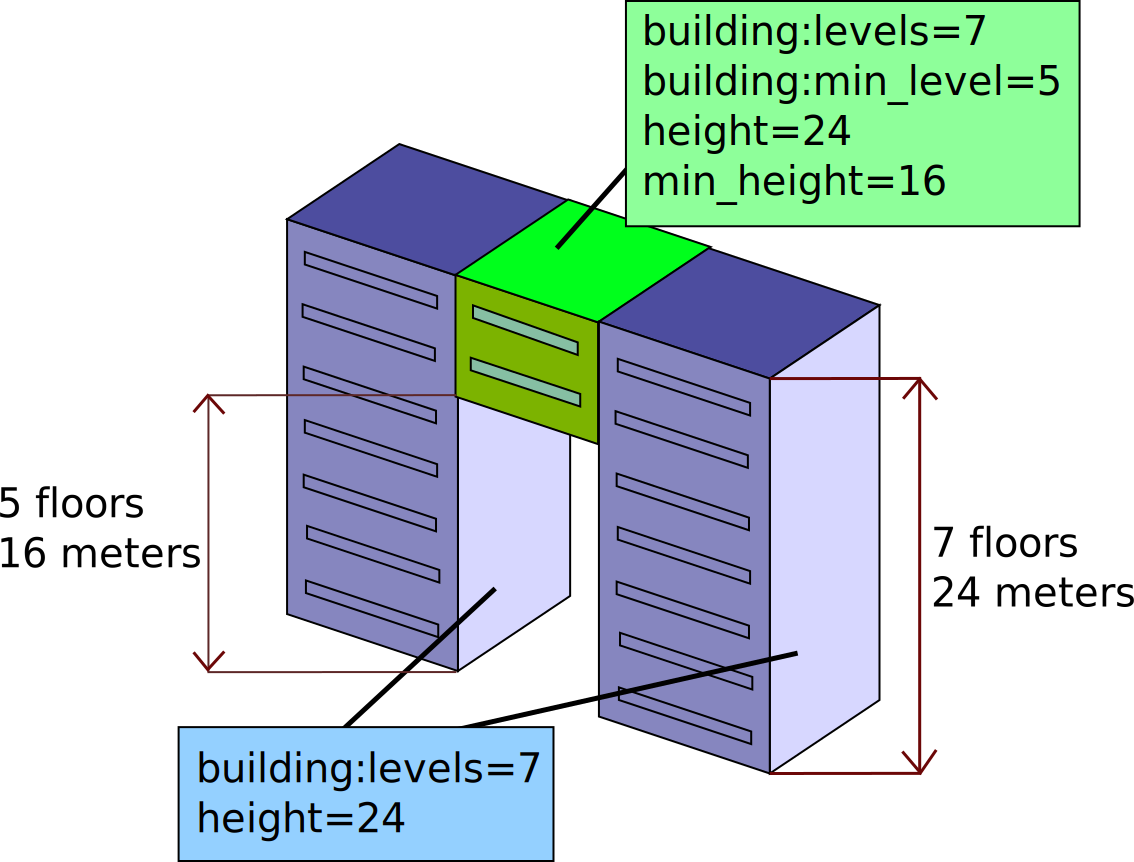
\includegraphics[width=0.55\textwidth]{assets/figures/Minlevel.svg}
    \caption{Hauteur minimum d'un bâtiment \cite{MinLevel-image}}
    \label{fig:building-Minlevel}
\end{figure}

La hauteur connue, on peut la transmettre à la classe \texttt{GltfBuilder} pour donner la hauteur au bâtiment lors de sa modélisation.

\subsection{glTF par bâtiment ou par tuile}

Quand on pense aux manière de générer les fichiers 3D, il est facile de concevoir que deux méthodes sont possibles : générer un fichier glTF par bâtiment ou générer un fichier glTF par tuile. La première méthode nous permettrait de générer des features par bâtiment glTF, ce qui rendrait l'utilisation de metadata très intéressante.

Plus intéressant encore, générer ces fichiers 3D par bâtiment nous pousserai fortement à tenir une liste de bâtiments se trouvant dans chaque tuile. En faisant ainsi, il serait possible de prévenir le placement d'un même bâtiment dans plusieurs tuiles. Souvent, un bâtiment se trouve à cheval sur plusieurs tuiles et il est donc nécessaire de le placer dans plusieurs fichiers glTF quand on génère un fichier par tuile.

Pour pouvoir générer un fichier glTF par bâtiment, il faut utiliser le concept de \textit{Multiple Content} introduit dans la version 1.1 de la spécification 3D Tiles \cite{3d-tiles-reference-card-v1_1}. Pour utiliser cela, il faut remplacer le champ \texttt{content} de chaque tuile par un champ \texttt{contents} qui sera une liste de plusieurs \texttt{content}. Chaque \texttt{content} contiendra un \texttt{uri} qui pointera vers le fichier glTF du bâtiment.

Cependant, un problème survient si l'on utilise en même temps l'implicit tiling lors de la génération des \textit{Subtrees}. Ces Subtrees, définis plus en profondeur dans leur chapitre dédié, nécessitent une liste de disponibilité (\autoref{sec:availability-class}) \textbf{par content}. En d'autres termes, si une tuile contient $X$ bâtiments, il faudra $X$ listes de disponibilité sur la tuile. Sur chacune de ces listes, une seule valeur sera à \texttt{true}, la valeur correspondant à l'index de la tuile sur laquelle le bâtiment se trouve. Cela rend donc la génération des Subtrees beaucoup plus complexe et énormément plus volumineuse.

\section{Database}
\label{sec:database}
La base de donnée \href{https://postgis.net/}{PostGIS}\footnote{https://postgis.net/} que j'utilise se distingue par deux catégories de tables différentes. Premièrement, il y a les tables qui on été générées par l'import de données OSM. Ces tables contiennent les informations des éléments OSM tels que les bâtiments, les routes, les rivières, etc. Deuxièmement, il y a les tables qui sont générées par mon application qui stockeront les tuiles 3D ainsi que les Subtrees pour éviter de les re-générer à chaque fois car cela peut prendre plusieurs heures si le dataset est grand.

Pour accéder aux données de ces tables, j'utilise la librairie java \texttt{javax.sql.DataSource} qui me permet de me connecter à la base de données.

\subsection{Données OSM}

Dans les données OSM, les parties qui nous intéresse sont les tables \texttt{osm\_nodes} et \texttt{osm\_relations}. Ces tables contiennent les données de tout les bâtiments. Ceux-ci ne contiennent généralement qu'une \Gls{géométrie}, une structure de donnée contenant plusieurs points et formant un polygone. Parfois seulement, des \Gls{tags} peuvent être ajoutés. Ces tags peuvent contenir des informations sur la hauteur du bâtiment, sa couleur, son matériau, etc.

La \href{https://wiki.openstreetmap.org/wiki/Simple_3D_Buildings}{documentation OpenStreetMap}\footnote{https://wiki.openstreetmap.org/wiki/Simple\_3D\_Buildings} nous permet d'avoir la liste complète des tags existants et nous intéressant concernant les bâtiments.

Pour pouvoir récupérer toutes ces informations, j'utilise la requête SQL suivante :

\newpage
\begin{verbatim}
SELECT st_asbinary(geom),
    tags -> building,
    tags -> height,
    tags -> building:levels,
    tags -> building:min_level,
    tags -> building:colour,
    tags -> building:material,
    tags -> building:part,
    tags -> roof:shape,
    tags -> roof:levels,
    tags -> roof:height,
    tags -> roof:color,
    tags -> roof:material,
    tags -> roof:angle,
    tags -> roof:direction
FROM osm_ways
WHERE (tags ? building or tags ? building:part) and
    st_intersects(geom, st_makeenvelope(%1$s, %2$s, %3$s, %4$s, 4326))
UNION
SELECT st_asbinary(geom),
    tags -> building,
    tags -> height,
    tags -> building:levels,
    tags -> building:min_level,
    tags -> building:colour,
    tags -> building:material,
    tags -> building:part,
    tags -> roof:shape,
    tags -> roof:levels,
    tags -> roof:height,
    tags -> roof:color,
    tags -> roof:material,
    tags -> roof:angle,
    tags -> roof:direction
FROM osm_relations
WHERE (tags ? building or tags ? building:part) and
    st_intersects(geom, st_makeenvelope(%1$s, %2$s, %3$s, %4$s, 4326));
\end{verbatim}

Grâce à cette requête, je récupère toutes les informations nécessaires pour définir et générer les bâtiments en fichiers glTF. \texttt{\%1\$s, \%2\$s, \%3\$s, \%4\$s, et \%5\$s} sont des espaces réservés qui seront remplacés par les coordonnées de la zone à charger lors de l'exécution de la requête.

\newpage
\subsection{Données générées}

Les données générées sont stockées dans les tables \texttt{td\_subtrees} et \texttt{td\_tile\_gltf}. La première contient toutes les informations nécessaires à la définition d'un Subtree. La seconde contient les fichiers glTF des tuiles. Ces tables sont définies comme suit :

\begin{verbatim}
CREATE TABLE td_subtrees
(
    morton_index bigint,
    level        integer,
    binary_file  bytea,
    UNIQUE (morton_index, level)
);

CREATE TABLE td_tile_gltf
(
    x           bigint,
    y           bigint,
    level       integer,
    gltf_binary bytea,
    UNIQUE (x, y, level)
);
\end{verbatim}

\chapter{Subtrees}

\section{Introduction}
\label{sec:subtrees-intro}
Lorsqu'on utilise l'implicit tiling, le client Cesium à besoin de recevoir en premier lieu une liste de tuiles disponibles. Cette liste doit lui être donnée sous forme de Subtree. Les \textit{Subtrees} dans Cesium constituent une composante essentielle pour la gestion et l'optimisation de la visualisation des données géospatiales volumineuses. Plutôt que de charger l'intégralité des données géospatiales, les Subtrees ont pour but d'indiquer au client Cesium quelles tuiles sont disponibles, quelles tuiles ont un contenu à afficher quelles sont ses enfants (\texttt{children}). Pour chacune de ces trois informations, un Subtree contient un objet \textit{Availability} (\autoref{sec:availability-class}) stockant une liste de boolean représentant chaque tuile. Pour savoir quel index de cette liste correspond à quelle tuile, un autre style de \textit{Binary Space Partitioning} est utilisé. Une \href{https://en.wikipedia.org/wiki/Z-order\_curve}{\textit{Z-order curve} ou un \textit{Morton order}}\footnote{https://en.wikipedia.org/wiki/Z-order\_curve} est utilisé pour définir les indexes (\autoref{sec:morton}).

Une fois ces Subtrees générés, il faudra les envoyer au client. Cela se fera en les transformant en JSON puis en un fichier respectant le \href{https://github.com/CesiumGS/3d-tiles/tree/main/specification/ImplicitTiling\#subtree-binary-format}{\textit{Subtree Binary Format}}\footnote{https://github.com/CesiumGS/3d-tiles/tree/main/specification/ImplicitTiling\#subtree-binary-format}

\subsection*{Hiérarchie de Subtrees}

\begin{figure}[H]
    \centering
    \includegraphics[width=1\textwidth]{assets/figures/Subtree_hierarchy.drawio.pdf}
    \caption{Exemple de hiérarchie de Subtrees}
    \label{fig:subtree-hierarchy}
\end{figure}

Le Tileset est partitionné en Subtrees de taille \texttt{subtreeLevels} fixe. Leur schéma de subdivision suit la même logique que les tuiles d'un implicit tiling. Chaque \textit{level} ou niveau représente une subdivision de la tuile de niveau inférieur. Un Subtree est généralement composé de plusieurs niveau de profondeur. Chaque niveau est composé d'une liste de noeuds représentant la disponibilité d'une tuile. En fonction du schema de subdivision, quadtree ou octree, chaque noeuds peut avoir 4 ou 8 enfants respectivement. On peut retrouver ces noeuds dans les listes de disponibilités citées plus haut. Les \textit{Availabilities} seront traités plus en détails dans la section \ref{sec:availability-class}.

Plusieurs Subtrees peuvent être liés entre eux pour former un arbre de Subtrees. Leur liaison se fait entre le noeuds \textit{root} d'un subtree et un noeuds au niveau maximum d'un autre Subtree. Par soucis de compréhension, j'appellerai le \textit{rang}, ou \textit{rank} en Anglais, d'un Subtree le niveau de profondeur de ce Subtree par rapport à la racine du Tileset. Le Subtree de rang 0 est le Subtree de la racine du Tileset. Les Subtree de rang maximum sont les Subtrees qui contiendront les contenus à afficher.

Finalement, quelques règles doivent être respectées lors d'une construction d'une hiérarchie de Subtrees:

\begin{itemize}
    \item Les Subtrees doivent être de même taille.
    \item Les Subtrees doivent avoir le même schéma de subdivision.
    \item Un Subtree doit contenir au minimum un niveau.
\end{itemize}

\newpage
\subsection*{Utilité des Subtrees}

Comme dit précédemment, les Subtrees sont utilisés pour indiquer au client Cesium quelles tuiles sont disponibles, quelles tuiles ont un contenu à afficher et quelles sont ses enfants. Ainsi, ils réduisent la quantité de données que le client Cesium demandera à l'API.

Dans la figure \ref{fig:subtree-debug} ci-dessous, vous pouvez observer le partitionnement binaire de l'espace grâce aux lignes de debug de l'application Cesium. Ces lignes suivent le partitionnement binaire que le client Cesium déduit des Subtrees qu'il à reçu. Là où se trouve des bâtiments, l'espace est plus subdivisé.

\begin{figure}[H]
    \centering
    \includegraphics[width=1\textwidth]{assets/figures/Subtree_debug.png}
    \caption{Partitionnement binaire de l'espace}
    \label{fig:subtree-debug}
\end{figure}

Pour comprendre ce que cela signifie, je fais une parallèle avec la section \ref{sec:lod} où j'ai mentionné les niveaux de détails. Il faut comprendre que chacun de ces subdivision est une tuile. Plus une tuile est subdivisée, plus elle elle correspond à un niveau bas dans la hiérarchies du tuilage, plus son contenu est détaillé. J'ai mentionné auparavant que ces niveaux de détails sont définis par la valeur \texttt{geometricError} d'une tuile. c'est toujours le cas. Le client Cesium suit une procédure très simple :

\begin{itemize}
    \item Le client charge une tuile disponible.
    \item Le client calcule le \texttt{Screen Space Error} (SSE) de cette tuile.
    \item Si le seuil SSE est dépassé et que les tuiles enfant sont disponibles, le client charge les tuiles enfant.
\end{itemize}

Ainsi, les tuiles sont chargées en fonction de leur disponibilité fournie par les Subtrees ainsi que leur \texttt{geometricError} et leur distance à la caméra.

\newpage
Un détail très important avec mon implémentation est que les niveaux des Subtrees et des listes de disponibilités sont complètement paramétrables. Actuellement, une seule restriction s'applique :  le contenu affichable ne peut se trouver que dans les Subtree de rang maximal (cf. \autoref{fig:subtree-hierarchy}). J'ai initialement rajouté cette restriction pour forcer l'utilisateur des fonction à garder une structure de la hiérarchie des Subtrees simple, néanmoins elle peut être facilement enlevée si voulu. Pour revenir à la paramétrisation des niveaux des Subtrees, il est possible de définir combien de niveaux contient un Subtree ainsi que le nombre de niveaux le tuilage entier comporte. Ces valeurs doivent être modifiées dans les fichiers :

\texttt{src/main/java/org/apache/baremaps/server/TdTilesResources.java}

et

\texttt{src/main/resources/tdtiles/tileset.json}

Parmi les autres paramètres modifiables, on trouve la possibilité de définir à partir de quels niveaux les tuiles contiennent un certain niveau de détails.

Il est donc possible d'alterner entre une subdivision ayant énormément de niveaux où le contenu ne s'affiche que pour de toutes petites tuiles et une subdivision ayant peu de niveaux où le contenu s'affiche pour des tuiles plus grandes. Cela permet de s'adapter aux tailles de scènes à afficher.

\section{Subtree Class}
\label{sec:subtree-class}
La première classe écrite dans le but de gérer les Subtrees est la classe \texttt{Subtree}. Un objet de cette classe comporte tout 

\section{Morton Index}
\label{sec:morton}
Le Morton index, également connu sous le nom \href{https://en.wikipedia.org/wiki/Z-order\_curve}{\textit{Z-Order Curve}}\footnote{{https://en.wikipedia.org/wiki/Z-order\_curve}}, est une technique d'encodage spatiale utilisée dans le contexte de l'implicit tiling. Cette méthode permet de convertir des coordonnées multidimensionnelles en une valeur unidimensionnelle tout en préservant la proximité spatiale des points. Dans le cas de Cesium, le Morton index facilite le découpage et l'organisation hiérarchique des tuiles, rendant plus efficace la gestion et le rendu des grandes quantités de données géospatiales. En encodant les coordonnées des tuiles dans une structure arborescente, le Morton index permet une récupération rapide des tuiles nécessaires pour afficher une vue spécifique, optimisant ainsi les performances et la fluidité de la visualisation.

Il y a plusieurs opérations sur les indexes de Morton qui sont nécessaires pour la gestion des tuiles. Ces opérations sont les suivantes :

\begin{itemize}
    \item Convertir des coordonnées (X, Y, Level) en un index de Morton.
    \item Convertir un index de Morton en des coordonnées (X, Y, Level).
    \item Obtenir les 4 indexes enfants d'un index de Morton.
\end{itemize}

\subsection*{Conversion de coordonnées en index de Morton}

Pour convertir des coordonnées (X, Y, Level) en un index de Morton, nous devons les \textit{intercaler} pour former un seul entier. L'intercalation des bits est une technique qui consiste à mélanger les bits de deux entiers pour former un index de Morton. Supposons que nous ayons deux entiers \( X \) et \( Y \), et que nous voulons les combiner en un seul entier \( Z \) en intercalant leurs bits.

1. \textbf{Représentation binaire}

   Tout d'abord, convertissons \( X \) et \( Y \) en leurs représentations binaires :
   \[
   X = x_n x_{n-1} \ldots x_1 x_0
   \]
   \[
   Y = y_n y_{n-1} \ldots y_1 y_0
   \]

2. \textbf{Intercalage des bits}

   Ensuite, nous intercalons les bits de \( X \) et \( Y \) pour obtenir \( Z \). Le bit \( i \) de \( X \) sera placé dans la position \( 2i \) de \( Z \), et le bit \( i \) de \( y \) sera placé dans la position \( 2i + 1 \) de \( z \). De plus, l'index de Morton dépend du niveau de profondeur de la tuile. Le nombre de bits nécessaires pour encoder un index de Morton est donc égal à \(2 \times \text{level}\).

   Formulons cela mathématiquement :
   \[
   Z = \text{interleave}(x, y) = z_{2n+1} z_{2n} z_{2n-1} \ldots z_1 z_0
   \]
   où
   \[
   z_{2i} = x_i \quad \text{et} \quad z_{2i+1} = y_i \quad \text{pour} \quad i = 0, 1, \ldots, n \quad \text{avec} \quad n = 2 \times {level}
   \]

   \newpage
3. \textbf{Exemple}

   Prenons un exemple simple avec \( x = 5 \) et \( y = 3 \). En binaire, nous avons :
   \[
   x = 101_2 \quad \text{et} \quad y = 011_2
   \]

   Intercalons les bits :
   \[
   z = 011011_2
   \]

   En décimal, cela donne :
   \[
   z = 27_{10}
   \]

Ainsi, l'index de Morton pour \( x = 5 \) et \( y = 3 \) est \( 27 \).

\begin{figure}[H]
    \centering
    \includegraphics[width=0.6\textwidth]{assets/figures/global-to-local-xy.png}
    \caption{Indexes X Y vers index de Morton \cite{availability-gh}}
    \label{fig:xy-morton}
\end{figure}

\subsection*{Conversion d'un index de Morton en coordonnées}

Le processus inverse du \textit{interleaving bits} consiste à séparer les bits d'un index de Morton \( Z \) pour récupérer les deux entiers \( X \) et \( Y \).

1. \textbf{Représentation binaire} :

   Supposons que nous avons un entier \( Z \) et que nous voulons en extraire les deux entiers \( X \) et \( Y \). Représentons \( Z \) en binaire :
   \[
   Z = z_{2n+1} z_{2n} z_{2n-1} \ldots z_1 z_0
   \]

   \newpage
2. \textbf{Séparation des bits} :

   Nous séparons les bits de \( Z \) pour reconstruire \( X \) et \( Y \). Les bits pairs de \( Z \) formeront \( X \), et les bits impairs de \( Z \) formeront \( Y \).

   Formulons cela mathématiquement :
   \[
   X = x_n x_{n-1} \ldots x_1 x_0
   \]
   \[
   Y = y_n y_{n-1} \ldots y_1 y_0
   \]

   où
   \[
   x_i = z_{2i} \quad \text{et} \quad y_i = z_{2i+1} \quad \text{pour} \quad i = 0, 1, \ldots, n \quad \text{avec} \quad n = 2 \times {level}
   \]

3. \textbf{Exemple} :

   Reprenons le dernier exemple avec \( Z = 27 \). En binaire, nous avons :
   \[
   Z = 011011_2
   \]

   Séparons les bits pour obtenir \( X \) et \( Y \) :
   \[
   X = z_{4}z_{2}z_{0} = 101_2 = 5_{10}
   \]
   \[
   Y = z_{5}z_{3}z_{1} = 011_2 = 3_{10}
   \]

Ainsi, les entiers \( X \) et \( Y \) extraits de l'index de Morton \( Z = 27 \) sont respectivement \( 5 \) et \( 3 \).

\subsection*{Obtention des indexes enfants}

Pour trouver les indexes enfants d'un index de Morton, nous devons simplement effectuer un décalage de 2 bits vers la gauche de l'index de Morton puis ajouter l'index de l'enfant voulu (de 0 à 3).

Par exemple, pour obtenir l'index de Morton de l'enfant 2 de l'index de Morton 27, nous effectuons les opérations suivantes :

\[
27 = 011011_2 \quad \Rightarrow \quad 01101100_2 = 108_{10}
\]

\[
108 + 2 = 110_{10} = 01101110_2
\]

Ainsi, l'index de Morton de l'enfant 2 de l'index de Morton 27 est 110.

\newpage
Une distinction qui se trouve parfois pratique est la distinction d'un index local avec un index global. Un index global est un index de Morton qui représente une tuile sur l'entièreté du Tileset, en comptant donc depuis l'index 0 du level 0. Tandis qu'un index local est un index de Morton qui représente une tuile avec pour référence l'index 0 du subtree.

\begin{figure}[H]
    \centering
    \includegraphics[width=0.8\textwidth]{assets/figures/global-to-local-morton.png}
    \caption{Index local et index global \cite{availability-gh}}
    \label{fig:morton-global-local}
\end{figure}

\section{Availabilities}
\label{sec:availability-class}
\input{tex-Subtrees/availabilities.tex}

\section{Transmission}
\label{sec:transmission}
Maintenant que nous savons comment les Subtrees sont créés, il ne reste plus qu'à savoir les transmettre au client Cesium. Ce client accepte sous deux formats différents. Nous pouvons soit lui envoyer la description du Subtree sous forme de JSON et lui envoyer les listes de disponibilités dans des fichiers binaires séparément en précisant les URI de ces fichiers dans le JSON. Comme seconde option, nous pouvons tout lui envoyer en un seul fichier binaire qui respecte le \href{https://github.com/CesiumGS/3d-tiles/tree/main/specification/ImplicitTiling#subtree-binary-format}{\textit{Subtree Binary Format}}\footnote{https://github.com/CesiumGS/3d-tiles/tree/main/specification/ImplicitTiling\#subtree-binary-format}. Sous ce format, les fichiers binaires sont inclus sous forme de buffer binaire. Les différentes listes de disponibilités pourront ensuite être retrouvées grâce à des offsets indiqués dans la partie JSON à la place des URI. Sauf raison externe, cette deuxième option est généralement plus simple à utiliser. C'est pourquoi je l'ai choisie pour mon implémentation.

Le \textit{Subtree Binary Format} est un format où les informations sont stockées en little-endian et dont les fichiers comportent un header de 24 Bytes. Ce header contient les informations suivantes :

\begin{figure}[H]
    \centering
    \includegraphics[width=1\textwidth]{assets/figures/binary-subtree.png}
    \caption{Header d'un fichier au \textit{Subtree Binary Format} \cite{implicit-tiling-gh}}
    \label{fig:xy-morton}
\end{figure}

Les informations contenues dans le header sont les suivantes :

\begin{itemize}
    \item \textbf{Magic} : 4 Bytes, \textit{magic number} identifiant ce fichier comme un Subtree. A toujours une valeur de \texttt{0x74627573}.
    \item \textbf{Version} : 4 Bytes, version du format binaire. Actuellement, le 24.07.2024, il s'agit de 1.
    \item \textbf{JSON Byte Length} : 8 Bytes, longueur de la partie JSON en Bytes.
    \item \textbf{Binary Byte Length} : 8 Bytes, longueur de la partie binaire en Bytes.
\end{itemize}

Concernant le \href{https://www.lalanguefrancaise.com/dictionnaire/definition/padding}\textit{padding}\footnote{https://www.lalanguefrancaise.com/dictionnaire/definition/padding}, les deux derniers éléments, \textit{JSON Byte Length} et \textit{Binary Byte Length}, doivent compter les Bytes de padding. Le padding est nécessaire car chaque chunk doit être aligné sur une frontière de 8 Bytes. La partie doit être remplie avec le caractère espace (\texttt{0x20}) sur la fin, tandis que la partie binaire doit être remplie avec des zéros (\texttt{0x00}) sur la fin.

\newpage
\subsection{Écriture de JSON}

Le JSON doit contenir les objets suivants :

\begin{itemize}
    \item \textbf{buffers} : une liste d'objet contenant le nom, les URI si nécessaire et la longueur des buffers binaires.
    \item \textbf{bufferViews} : une liste d'objet contenant les les offsets des différentes parties des buffers binaires.
    \item \textbf{tileAvailability} : un objet décrivant liste de disponibilités des tuiles.
    \item \textbf{contentAvailability} : un objet décrivant liste de disponibilités des contenus.
    \item \textbf{childAvailability} : un objet décrivant liste de disponibilités des enfants.
\end{itemize}

Les objets \texttt{buffer} doivent contenir les informations suivantes :

\begin{itemize}
    \item \textbf{name} : nom du buffer.
    \item \textbf{uri} : URI du fichier binaire, doit être omis si on utilise le \textit{Subtree Binary Format}.
    \item \textbf{byteLength} : longueur du fichier binaire.
\end{itemize}

Les objets \texttt{bufferViews} doivent contenir les informations suivantes :

\begin{itemize}
    \item \textbf{buffer} : index du buffer auquel le bufferView fait référence dans la liste de buffers.
    \item \textbf{byteOffset} : offset de la vue dans le buffer.
    \item \textbf{byteLength} : longueur de la vue.
\end{itemize}

Les objets \texttt{tileAvailability}, \texttt{contentAvailability} et \texttt{childAvailability} peuvent soit contenir un objet \texttt{constant} ayant une valeur de \texttt{0} ou \texttt{1} qui signifie que toutes les tuiles ont la même disponibilité. Soit contenir un objet \texttt{bufferView} qui fait référence à un bufferView contenant les listes de disponibilités avec un objet \texttt{availableCount} qui indique le nombre de tuiles disponibles.

\begin{itemize}
    \item \textbf{constant} : objet contenant une valeur de \texttt{0} ou \texttt{1}.
    \item \textbf{bufferView} : index du bufferView contenant les listes de disponibilités.
    \item \textbf{availableCount} : nombre de tuiles disponibles.
\end{itemize}

D'autres informations peuvent notamment être ajoutées au JSON tel que des metadata.

Voici un exemple de JSON d'un des Subtrees créés par mon implémentation :

\begin{verbatim}
    TODO
\end{verbatim}

\chapter{Conclusion}
\label{sec:conclusion}
%%if
% Bien que non nécessaire dans un rapport de Bachelor, la discussion finale d'un projet résume les résultats obtenus et dresse une conclusion objective du projet. Un manager de société est souvent amené à lire de nombreux rapport, il ne s'intéresse généralement qu'à l'introduction au contexte de l'étude et à sa conclusion.

% Si nécessaire, n'hésitez pas à scinder votre conclusion en deux parties : une conclusion technique et une conclusion personnelle.

% Il est de coutume de signer la conclusion...
%%fi

Pour conclure, ce travail a permis de mettre en place un prototype d'une utilisation du client Cesium pour afficher des bâtiments venant d'OpenStreetMap en 3D. Ce prototype a démontré qu'il était possible d'utiliser la fonctionnalité d'implicit tiling de la spécification 3D Tiles Next tout en gardant un résultat satisfaisant et qu'il était possible de le faire en traitant les données de manière uniforme pour l'entièreté du dataset d'OpenStreetMap.

La génération des Subtrees est maintenant totalement fonctionnelle. Cette génération est régie par des paramètres pouvant changer intégralement la forme de la hiérarchie des Subtrees. Cela permet d'adapter à souhait quels niveaux de la division par implicit tiling contiendra du contenu 3D ainsi que de préciser leur niveaux de détails.

Actuellement, ce prototype est parfaitement utilisable à condition de passer un peu de temps à trouver les bons niveaux de compression des géométries des bâtiments 3D et les bons niveaux auxquels appliquer ces compression. Pour cela, de nombreuses mesures doivent être prises sur différentes plateformes pour trouver le bon compromis entre qualité et performance. Autant cruciale qu'elle l'est, cette étape sort du carde de ce travail. Elle reste donc à être effectuée.

Un autre point qui semble être la prochaine étape logique du développement de ce projet est l'amélioration de la génération des objets glTF représentant les bâtiments. Beaucoup d'informations sont mises à dispositions par le dataset proposé par OpenStreetMap. Comme expliqué dans le rapport du travail de Bachelor mentionné dans la section \ref{sec:gltf}, il est possible de pousser la génération des bâtiments plus loin en intégrant leur toit ou en ajoutant des textures. Mais ce rapport montre aussi qu'il est possible de générer bien plus que des bâtiments, comme les routes ou la végétation.

\vfil
\hspace{8cm}\makeatletter\@author\makeatother\par
\hspace{8cm}\begin{minipage}{5cm}
    %%if
    % Place pour signature numérique
    \printsignature
    %%fi
\end{minipage}

\clearpage
\printbibliography

\appendix
\appendixpage
\addappheadtotoc

%%if
% \chapter{Première annexe}

% Les annexes n'ont pas un contenu \underline{normatif} mais \underline{descriptif}. Tout contenu annexé ne doit pas être nécessaire à la bonne compréhension du travail.

% Les annexes contiennent généralement :

% \begin{itemize}
%     \item les dessins mécaniques (mises en plan);
%     \item les schémas électriques détaillés;
%     \item des photographies du projet;
%     \item des scripts et des extraits de code source;
%     \item des documents techniques \pex \emph{datasheet};
%     \item des développements mathématiques.
% \end{itemize}
% \section{Sous section}
% \lipsum[1]
%%fi

\let\cleardoublepage\clearpage
\backmatter

\label{glossaire}
\printnoidxglossary
\label{index}
\printindex

% Le colophon est le dernier élément d'un document qui contient des notes de l'auteur concernant la mise en page et l'édition du document : il est parfaitement optionnel.
% \input{colophon.tex}

\end{document}